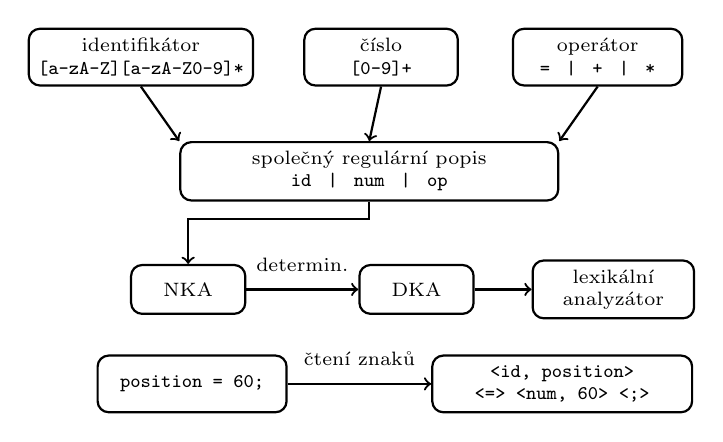
\begin{tikzpicture}[
    box/.style={
        draw,
        rounded corners,
        thick,
        align=center,
        font=\scriptsize,
        minimum height=0.72cm
    },
    smallbox/.style={
        draw,
        rounded corners,
        thick,
        align=center,
        font=\scriptsize,
        minimum width=1.45cm,
        minimum height=0.62cm
    },
    arrow/.style={->, thick}
]

    % horní řada: regulární výrazy tokenů
    \node<2->[box, minimum width=2.45cm] (re1) at (0,0)
        {identifikátor\\\texttt{[a-zA-Z][a-zA-Z0-9]*}};

    \node<2->[box, minimum width=1.95cm] (re2) at (3.05,0)
        {číslo\\\texttt{[0-9]+}};

    \node<2->[box, minimum width=2.15cm] (re3) at (5.80,0)
        {operátor\\\texttt{= \;|\; + \;|\; *}};

    % mezikrok: společný regulární popis
    \node<3->[box, minimum width=4.8cm] (combined) at (2.90,-1.45)
        {společný regulární popis\\
        \texttt{id \;|\; num \;|\; op}};

    \draw<3->[arrow] (re1.south) -- (combined.north west);
    \draw<3->[arrow] (re2.south) -- (combined.north);
    \draw<3->[arrow] (re3.south) -- (combined.north east);

    % konstrukce automatů
    \node<4->[smallbox] (nfa) at (0.60,-2.95) {NKA};
    \node<5->[smallbox] (dfa) at (3.50,-2.95) {DKA};
    \node<6->[box, minimum width=2.05cm] (lexer) at (6.00,-2.95)
        {lexikální\\analyzátor};

    \draw<4->[arrow] (combined.south) -- ++(0,-0.225) -| (nfa.north);
    \draw<5->[arrow] (nfa) -- node[above, font=\scriptsize, yshift=1mm] {determin.} (dfa);
    \draw<6->[arrow] (dfa) -- (lexer);

    % spodní ukázka
    \node<7->[box, minimum width=2.4cm] (src) at (0.65,-4.15)
        {\texttt{position = 60;}};

    \node<7->[box, minimum width=3.3cm] (tok) at (5.35,-4.15)
        {\texttt{<id, position>}\\
        \texttt{<=> <num, 60> <;>}};

    \draw<7->[arrow] (src) -- node[above, font=\scriptsize, yshift=1mm] {čtení znaků} (tok);

\end{tikzpicture}
